    \documentclass[]{standalone}
    \usepackage{tikz}
    \usetikzlibrary{calc}
    
    \begin{document}
    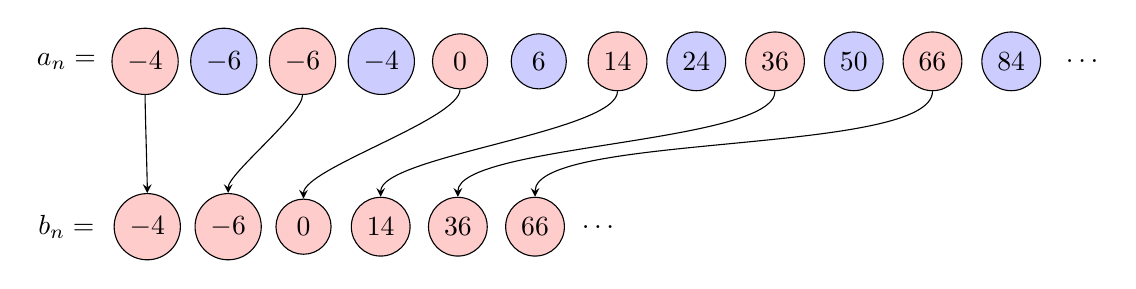
\begin{tikzpicture}
    	\tikzset{element/.style={draw=black, anchor=west, circle, minimum size=7mm, fill=#1}}
    	
    	% Sequence a_n
    	\node (a0) at (0,0) {$a_{n}=$};
    	\foreach \n in {1,...,12}{
    		\pgfmathsetmacro{\ai}{int(\n^2-5*\n)}
    		\pgfmathsetmacro{\m}{int(\n-1)}
    		\pgfmathsetmacro{\c}{int(mod(\n,2))}
    		\ifnum \c=1
    			\def\col{red}
    		\else
    			\def\col{blue}
    		\fi
    		\node[element={\col!20}, right of=a\m] (a\n) {$\ai$};
    	}
    	\node[right of=a12, xshift=-1mm] (dots1) {$\dots$};
    	
    	% Subsequence b_n
    	\tikzset{node distance=6mm}
    	\node[below of=a0, yshift=-15mm] (b0) {$b_{n}=$};
    	\foreach \n in {1,...,6}{
    		\pgfmathsetmacro{\bi}{int((2*\n-1)^2-5*(2*\n-1))}
    		\pgfmathsetmacro{\m}{int(\n-1)}
    		\pgfmathsetmacro{\k}{int(2*\n-1)}
    		\node[right of=b\m, element={red!20}] (b\n) {$\bi$};
    		\draw[-stealth] (a\k.south) to [out=-90, in=90, looseness=0.4] (b\n.north);
    	}
    	\node[right of=b6, xshift=2mm] (dots2) {$\dots$};
    \end{tikzpicture}
    \end{document}
